\headline{{\textbf{\Large\sffamily Bonsai Roots:}}\\
{\textbf{\large\sffamily Meet the Members of TWBC}}}
\phantomsection
\label{2026-01-roots}
\noindent
In every edition of \emph{Bonsai Roots}, we pause from wiring, watering, and weekend workshops to celebrate the people who shape our club.
Each story adds character to the ever\--growing forest of TWBC.
This month, we are delighted to introduce a member whose passion for the craft is matched only by her dedication to the community: \textbf{Liz Panton}!

\begin{itemize}
    \item \textbf{What's your name and where in the country do you live?}\\
    \emph{My name is Liz Panton. I live in Fittleworth, West Sussex. I am an online member of TWBC and Chairman of Chichester and District Bonsai Society, though I stay active with the UK Bonsai Association steering group.}

    \item \textbf{What are your favourite species of tree and why?}\\
    \emph{I love Korean Hornbeam for their small leaves, Maples for their variety, and Satsuki Azaleas for those heart-warming flowers. Each species offers a unique challenge that keeps me busy all year round.}

    \item \textbf{What aspect of bonsai do you enjoy?}\\
    \emph{So many things! I love learning new techniques, making friends, and the meditative focus it provides. It’s a wonderful way to forget the world and achieve a true sense of accomplishment.}

    \item \textbf{What aspects of bonsai do you find most challenging?}\\
    \emph{I struggle with the artistic side and, being partially dyslexic, I have to do things repeatedly to remember them. Also, as I get older, moving the heavier trees is becoming quite the physical challenge!}

    \begin{minipage}[b]{0.45\textwidth}
        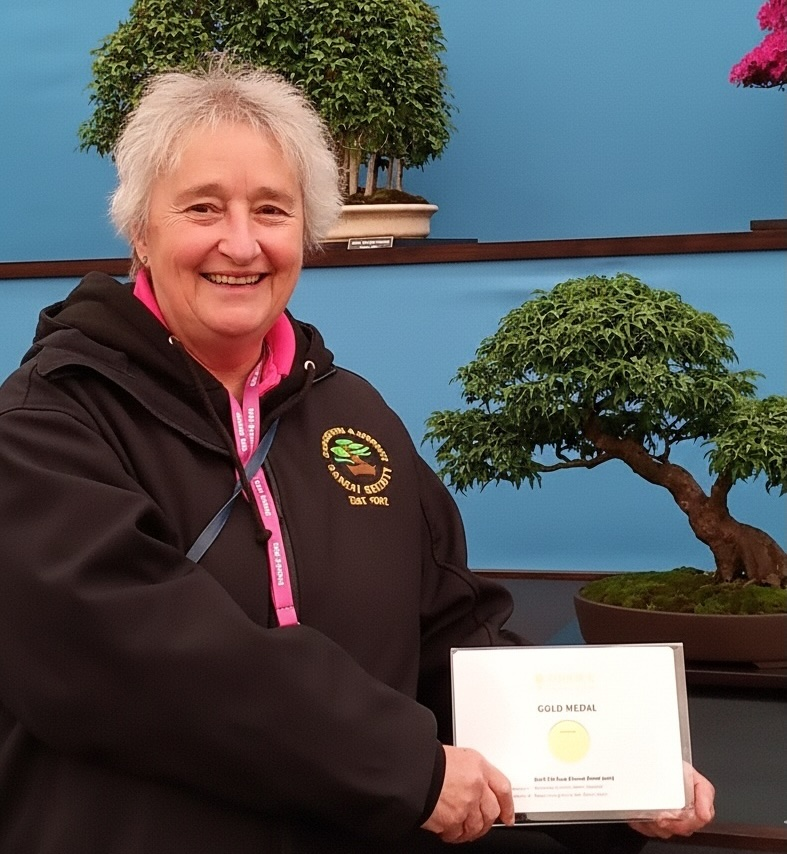
\includegraphics[angle=0,origin=c,width=1.0\textwidth]{2026_01/res/2601_roots_liz_panton}
        \centerline{\emph{Liz with her prize-winning Shishigashira Maple.}}
    \end{minipage}
%    \columnbreak

    \item \textbf{Who or what inspires you throughout your bonsai journey?}\\
    \emph{My husband has been my biggest supporter; he bought me my first tree 30 years ago. I’ve loved trees since childhood, even winning the Observers Book of Trees at school!}

    \item \textbf{How long have you been interested in keeping bonsai?}\\
    \emph{I have been practicing for over 30 years. I started at the Little Oak School of Bonsai, and some of the trees I styled back then have now matured into amazing show-quality bonsai.}

    \item \textbf{What stimulated your interest in bonsai?}\\
    \emph{The people! Whether it’s sharing ideas or seeing a tree win `Best in Show' when I didn't think it was ready. I even became Chairman of my local club to help it grow and evolve.}

    \item \textbf{If you could give someone new to bonsai any tips, what would it be?}\\
    \emph{Join a club! Practicing bonsai alone can be very lonely. Join as many as you like: every club is different and provides invaluable guidance and a place to bounce ideas around.}

    \item \textbf{Why do you enjoy being part of TWBC, and do you have any ideas or suggestions for the club's future?}\\
    \emph{I owe TWBC a huge debt. Just after COVID, an invite to show my Maple here led to it being featured at the Chelsea Flower Show! This club literally changed my life and gave me so much confidence.}

    \item \textbf{One word to describe what bonsai means to you?}\\
    \emph{Aspirational! Though honestly, one word is never enough to describe what this hobby means to me.}

    \item \textbf{What are your future goals regarding your own trees and learning more about the hobby?}\\
    \emph{I want to keep learning, though I need to thin out my collection. My neighbor is leaving me 30 mature trees in his will, so I’m going to need a lot more space soon!}

    \item \textbf{How would you like to see your bonsai journey progress in the future?}\\
    \emph{I hope to meet more friends, learn from the experts, and encourage others to get involved in the hobby. Most of all, I just want to have fun and enjoy the journey.}
\end{itemize}

Liz's story is a beautiful reminder of how bonsai connects us across counties and clubs, turning small trees into life\--changing opportunities.
We are so grateful for her energy and her presence in our community.
Who will we meet next time?
Stay tuned for more in \emph{Bonsai Roots}!

\begin{center}
            $\cdots$
\end{center}

\noindent \emph{If you're a newer member and would like to feature in a future edition of Bonsai Roots, simply fill out the form at \href{https://forms.gle/quVXa4L8rhpnT5kr6}{this link}! We'd love to hear your story.}

\closearticle
\columnbreak
